\documentclass[11pt,letterpaper]{article}
\usepackage[spanish,es-noshorthands,es-tabla]{babel}
\usepackage[utf8]{inputenc}
\usepackage[T1]{fontenc}
\usepackage{lmodern}
\usepackage[margin=2.5cm]{geometry}
\usepackage{amsmath,amssymb}
\usepackage{graphicx}
\usepackage{booktabs}
\usepackage{tabularx}
\usepackage{float}
\usepackage{tikz}
\usetikzlibrary{positioning,arrows.meta}
\usepackage[hidelinks]{hyperref}
\usepackage{url}
\usepackage[spanish=mexican]{csquotes}
\usepackage[style=authoryear,natbib=true,maxcitenames=2,uniquelist=false,uniquename=false]{biblatex}
\addbibresource{referencias.bib}
\graphicspath{{../results/figures/}}

\newcommand{\autor}{Nombre del autor}
\newcommand{\carne}{Carn\'e 00000}

\begin{document}

\begin{titlepage}
\centering
{\large Universidad del Valle de Guatemala\par}
{\large CC3074 Modelizaci\'on y Simulaci\'on, ciclo 2 de 2026\par}
\vspace{3cm}
{\LARGE\bfseries Salida de p\'ublico al cierre de un concierto en la Explanada Cayal\'a\par}
\vspace{0.5cm}
{\large Fuerzas sociales y enjambre de part\'iculas para ubicar barras y vallas\par}
\vspace{3cm}
{\large Proyecto 2\par}
\vspace{1cm}
{\large \autor\par \carne\par}
\vfill
{\large Noviembre de 2026\par}
\end{titlepage}

\tableofcontents
\newpage

\section{Problema y delimitaci\'on}

\subsection{Contexto}
La Explanada Cardales de Cayal\'a, en la zona 16 de la Ciudad de Guatemala, es un espacio abierto que se usa para conciertos grandes. Para los conciertos de noviembre de 2022 las autoridades esperaban m\'as de 15 mil personas por d\'ia \citep{prensalibre2022}. Al terminar el concierto casi todo el p\'ublico sale al mismo tiempo. Una parte va primero a las barras cashless a comprar o a devolver saldo, y el resto camina directo a los portones. Las filas de las barras y el flujo hacia la salida se cruzan, y en esos puntos la gente se amontona.

Cuando la densidad pasa de unas 4 personas por metro cuadrado el contacto f\'isico se vuelve inevitable y la circulaci\'on casi se detiene \citep{fruin1971}. Por eso la ubicaci\'on de barras y vallas no es un detalle de decoraci\'on: decide d\'onde se forman los tapones.

\subsection{Zona modelada}
No se modela toda la explanada sino la zona cr\'itica de salida. En OpenStreetMap no existe un elemento llamado ``Explanada Cayal\'a''. Se usa el lote abierto m\'as grande junto a Cardales de Cayal\'a (way 688526225, 8555 m$^2$) \citep{osm688526225}, que coincide con la ubicaci\'on de la ``Explanada Cardales'' que menciona la nota de prensa \citep{prensalibre2022}. Esta identificaci\'on es una suposici\'on del autor.

Sobre ese pol\'igono real se coloca una ventana de 80 por 50 metros en el extremo sur. El dominio es la intersecci\'on de ambos y mide 3145 m$^2$. Los bordes oeste y sur y la esquina recortada del sureste son bordes reales del lote. Los bordes norte y este son cortes de la ventana y se tratan como paredes. La Figura~\ref{fig:recinto} muestra el pol\'igono, la ventana y el montaje base.

\begin{figure}[H]
\centering
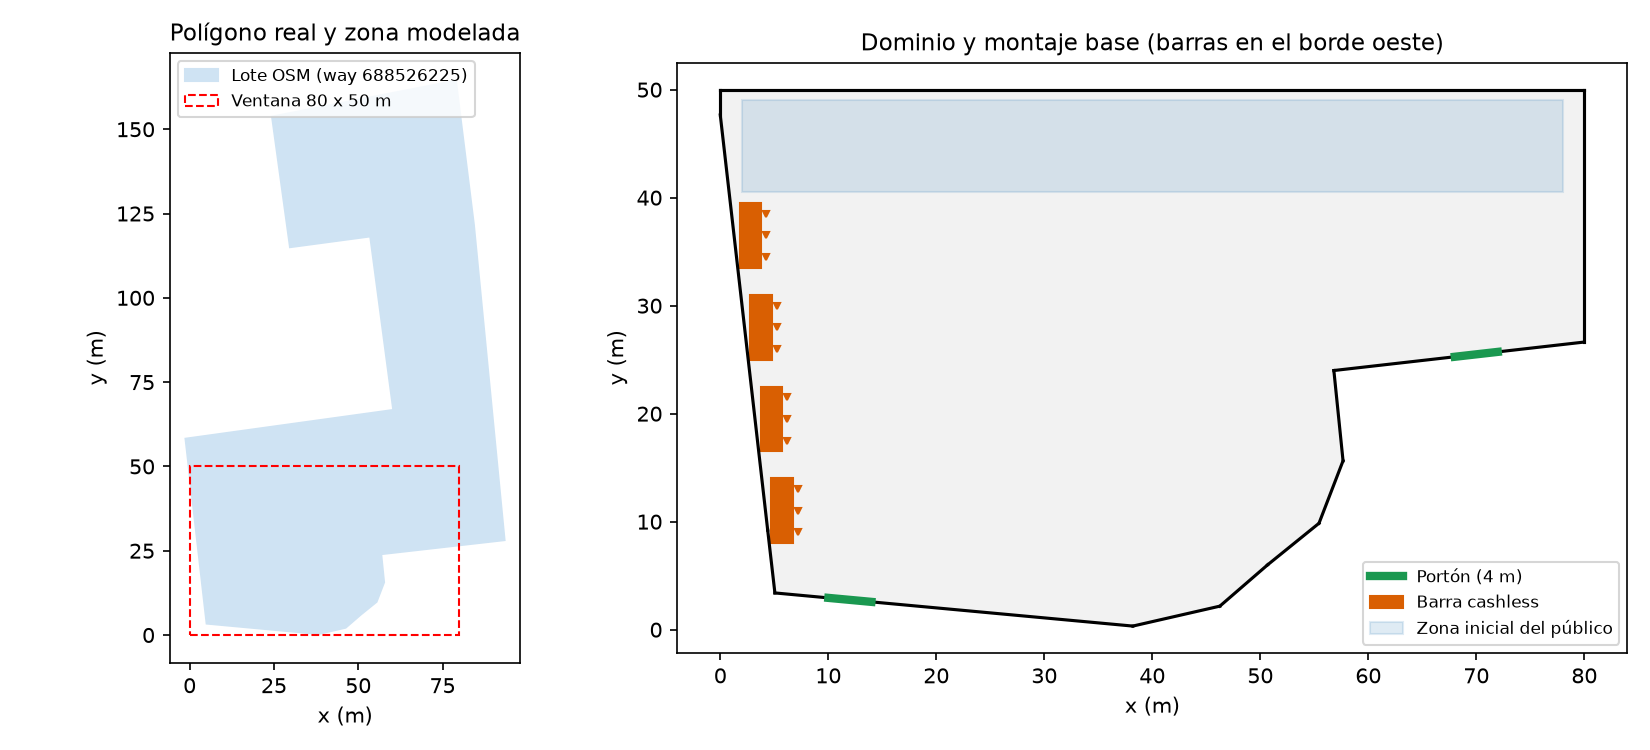
\includegraphics[width=\textwidth]{fig_recinto.png}
\caption{Izquierda: lote real de OpenStreetMap y ventana modelada. Derecha: dominio, portones, montaje base con las cuatro barras en el borde oeste y zona donde inicia el p\'ublico. Los tri\'angulos marcan los puntos de atenci\'on de cada barra.}
\label{fig:recinto}
\end{figure}

\subsection{Actores e interacciones}
\begin{itemize}
\item \textbf{Asistentes}: cada persona camina hacia su objetivo, evita a las dem\'as y evita paredes y mobiliario. El 35\,\% decide pasar por una barra.
\item \textbf{Barras cashless}: cuatro m\'odulos de 2 por 6 metros con tres puntos de atenci\'on cada uno. Cada punto atiende a una persona a la vez en orden de llegada.
\item \textbf{Vallas encauzadoras}: dos vallas met\'alicas de 6 metros que ordenan el flujo frente a los portones. El montaje base no las usa.
\item \textbf{Portones}: dos salidas de 4 metros de ancho en el borde sur.
\end{itemize}

\subsection{Pregunta de investigaci\'on}
?`En qu\'e porcentaje bajan la densidad pico y el tiempo de salida cuando la ubicaci\'on de barras y vallas se elige con un enjambre de part\'iculas, frente al montaje tradicional con las barras pegadas al borde oeste?

\subsection{Objetivos}
\begin{enumerate}
\item Ajustar el modelo de movimiento con datos reales de cuellos de botella de J\"ulich y reportar su error absoluto medio.
\item Encontrar con PSO una ubicaci\'on de barras y vallas que cumpla las restricciones de seguridad.
\item Medir con 30 r\'eplicas por condici\'on el cambio en densidad pico y tiempo de salida, con intervalos de confianza del 95\,\%.
\item Comprobar por c\'odigo que ning\'un mueble bloquea rutas de salida y que la densidad no pasa de 4 personas por m$^2$.
\end{enumerate}

\subsection{M\'etricas}
\begin{itemize}
\item \textbf{Densidad pico} $D_{\max}$ (personas/m$^2$, se busca bajarla): el valor m\'as alto en el tiempo y en el espacio del mapa de densidad suavizado, contando solo las zonas por donde se puede caminar.
\item \textbf{Tiempo de salida del 95\,\%} $T_{95}$ (s, se busca bajarlo): el instante en que el 95\,\% del aforo ya cruz\'o un port\'on.
\end{itemize}

\subsection{Entradas y salidas}
\begin{table}[H]
\centering
\begin{tabularx}{\textwidth}{lX}
\toprule
Entradas & Pol\'igono del recinto, posici\'on de barras y vallas, aforo, probabilidad de compra, tiempo medio de atenci\'on, semilla. \\
Salidas & Series de densidad en el tiempo, mapa de densidad m\'axima, tiempo de salida de cada persona, $D_{\max}$ y $T_{95}$. \\
\bottomrule
\end{tabularx}
\end{table}

\subsection{Supuestos y exclusiones}
Se supone terreno plano, buena iluminaci\'on y un cierre normal, sin p\'anico. Todo el p\'ublico modelado est\'a dentro de la zona al iniciar el cierre. Quedan fuera sismos, ri\~nas, lluvia, emergencias m\'edicas y el tr\'afico de veh\'iculos afuera del recinto. Tampoco se modelan ba\~nos ni otros servicios.

\subsection{Tipo de datos}
\begin{table}[H]
\centering
\begin{tabularx}{\textwidth}{llX}
\toprule
Dato & Tipo & Fuente \\
\midrule
Pol\'igono del lote & Real & OpenStreetMap, consulta del 8 de noviembre de 2026 \\
Ventana y posici\'on de portones & Estimaci\'on & Elecci\'on del autor sobre el pol\'igono real \\
Tama\~no de barras y vallas & Estimaci\'on & Medidas t\'ipicas de mobiliario de eventos \\
Posici\'on inicial y compras & Sint\'etico & Generado con semillas fijas \\
\bottomrule
\end{tabularx}
\end{table}

\section{Técnica investigada: enjambre de partículas}

\subsection{Idea y funcionamiento}
El enjambre de partículas (PSO) es un método de búsqueda inspirado en el movimiento de bandadas \citep{kennedy1995}. Cada partícula es una solución completa, en este caso un montaje de barras y vallas. Las partículas se mueven por el espacio de búsqueda y en cada paso combinan tres tendencias: seguir moviéndose en la misma dirección, volver hacia el mejor punto que ellas mismas han visto ($p_i$) y acercarse al mejor punto que ha visto todo el enjambre ($g$):
\begin{equation}
v_i^{k+1} = w^k v_i^k + c_1 r_1 (p_i - x_i^k) + c_2 r_2 (g - x_i^k), \qquad x_i^{k+1} = x_i^k + v_i^{k+1}
\end{equation}
donde $r_1$ y $r_2$ son números aleatorios uniformes entre 0 y 1, distintos para cada coordenada. El peso de inercia $w^k$ baja de 0.9 a 0.4 a lo largo de las iteraciones: al inicio las partículas recorren mucho terreno y al final afinan cerca de lo mejor encontrado \citep{shi1998}. Los coeficientes $c_1 = c_2 = 1.49$ están cerca del valor 1.49445 que \citet{clerc2002} mostraron que mantiene estable el movimiento del enjambre.

\subsection{Representación de una solución}
Cada partícula es un vector $x \in \mathbb{R}^{14}$: las coordenadas $(x, y)$ del centro de las cuatro barras (8 valores) y, para cada una de las dos vallas, su punto medio y su ángulo $\theta \in [-\pi/2, \pi/2]$ (6 valores). Las barras pueden ir a cualquier punto del rectángulo que contiene al recinto. Cada valla se limita a un cuadro de 16 por 16 metros frente a su portón (Tabla~\ref{tab:limites}).

El ángulo necesita un cuidado especial. Una valla girada $\pi/2$ es la misma que una girada $-\pi/2$, así que recortar el ángulo en los bordes partiría en dos una misma orientación. Por eso, cuando una partícula se pasa del borde en el ángulo, reaparece por el otro lado. En las coordenadas de posición sí se recorta y se anula la velocidad.

\begin{table}[H]
\centering
\caption{Límites de búsqueda de cada variable.}
\label{tab:limites}
\begin{tabular}{lrr}
\toprule
Variable & Mínimo & Máximo \\
\midrule
Barra 1 x (m) & 1 & 79 \\
Barra 1 y (m) & 3.33 & 47 \\
Barra 2 x (m) & 1 & 79 \\
Barra 2 y (m) & 3.33 & 47 \\
Barra 3 x (m) & 1 & 79 \\
Barra 3 y (m) & 3.33 & 47 \\
Barra 4 x (m) & 1 & 79 \\
Barra 4 y (m) & 3.33 & 47 \\
Valla 1 x (m) & 4.83 & 20.83 \\
Valla 1 y (m) & 3.72 & 19.72 \\
Valla 1 ángulo (rad) & -1.57 & 1.57 \\
Valla 2 x (m) & 60.98 & 76.98 \\
Valla 2 y (m) & 26.44 & 42.44 \\
Valla 2 ángulo (rad) & -1.57 & 1.57 \\
\bottomrule
\end{tabular}

\end{table}

\subsection{Procedimiento}
\begin{enumerate}
\item Crear 12 partículas en montajes válidos tomados al azar dentro de los límites (los inválidos se descartan) y con velocidad cero.
\item Evaluar cada partícula. Primero pasa por el validador geométrico; solo si es válida se simula.
\item Para cada iteración $k$ hasta 25: calcular $w^k$, actualizar velocidades con la ecuación anterior, limitar cada componente de la velocidad al 20\,\% del rango de esa variable, mover las partículas, aplicar los límites y evaluar.
\item Actualizar el mejor punto de cada partícula y el del enjambre.
\item Detenerse si el mejor valor del enjambre mejora menos de 0.001 durante 5 iteraciones seguidas.
\end{enumerate}

La regla de paro pedía detenerse cuando la mejora fuera menor a 0.001. Aplicada a una sola iteración, el método se detiene casi de inmediato, porque es normal que el mejor valor del enjambre no cambie en una iteración y sí cambie en la siguiente. Por eso se exigen 5 iteraciones seguidas sin mejora.

\subsection{Parámetros}
\begin{table}[H]
\centering
\caption{Parámetros del PSO.}
\begin{tabularx}{\textwidth}{llX}
\toprule
Parámetro & Valor & Justificación \\
\midrule
Partículas & 12 & Cada evaluación cuesta 3 simulaciones; 12 partículas por 25 iteraciones son 900 simulaciones por corrida. \\
Iteraciones & 25 & Presupuesto de cómputo de una corrida en una computadora personal. \\
Inercia $w$ & 0.9 a 0.4 & Valores de \citet{shi1998}. \\
$c_1$, $c_2$ & 1.49 & Cercanos al valor estable de \citet{clerc2002}. \\
Velocidad máxima & 20\,\% del rango & Evita que las partículas salten de un borde al otro. \\
Paro & mejora $<$ 0.001 en 5 iteraciones & Ver el procedimiento. \\
\bottomrule
\end{tabularx}
\end{table}

\subsection{Validador geométrico y restricciones}
Antes de simular, cada montaje pasa por un validador escrito para este proyecto. El recinto se divide en celdas de 0.25 por 0.25 metros y se revisan cinco reglas:
\begin{enumerate}
\item Ningún mueble sale del recinto.
\item Dos muebles no se tocan ni dejan entre sí un paso menor a 1.12 metros.
\item Ningún mueble entra en el círculo de 5 metros alrededor de cada portón.
\item Frente a la cara de atención de cada barra quedan 8 metros libres para la fila, fuera de ese círculo.
\item Desde toda zona por donde se camina se puede llegar a un portón por pasos de al menos 1.12 metros. Esto se comprueba con el algoritmo de Dijkstra sobre las celdas.
\end{enumerate}
Cada regla incumplida suma a la penalización $P_{\text{geom}}$ el área en metros cuadrados donde ocurre. Un montaje es válido solo si $P_{\text{geom}} = 0$. Si no lo es, no se simula y recibe $J = 2 + \lambda_{\text{geom}} P_{\text{geom}}$, que siempre es peor que cualquier montaje válido. Así el enjambre sabe cuánto se equivocó y hacia dónde corregir.

La Tabla~\ref{tab:factibilidad} muestra que solo el 3.3\,\% de los montajes tomados al azar cumplen todas las reglas. La regla que más falla es la de la zona de fila. La zona válida es pequeña y está partida en pedazos, por lo que en la búsqueda real el enjambre arranca con partículas válidas.

\begin{table}[H]
\centering
\caption{Montajes al azar frente al validador y búsqueda de un montaje válido con PSO.}
\label{tab:factibilidad}
\begin{tabular}{lr}
\toprule
Indicador & Valor \\
\midrule
Montajes al azar evaluados & 1000 \\
Montajes válidos (\%) & 1 \\
Con violación de fuera del recinto (\%) & 87 \\
Con violación de traslape o paso angosto (\%) & 29.1 \\
Con violación de radio libre de salida (\%) & 51.4 \\
Con violación de zona de fila (\%) & 95.8 \\
Con violación de área sin salida (\%) & 6 \\
Iteración en que PSO halla un montaje válido & 6 \\
\bottomrule
\end{tabular}

\end{table}

\subsection{Por qué PSO y no otra técnica}
La función que se quiere minimizar sale de una simulación con azar, colas y eventos discretos. No tiene derivadas y cambia un poco entre semillas, así que los métodos basados en gradiente no sirven. Entre los métodos que no usan derivadas, se eligió PSO por tres razones:
\begin{itemize}
\item Cada partícula se mueve de forma continua, así que un montaje cambia poco a poco y conserva su sentido geométrico. En un algoritmo genético el cruce mezcla coordenadas de montajes distintos y suele producir barras encimadas, lo que aquí es grave porque solo el 3.3\,\% del espacio es válido.
\item Tiene pocos parámetros y valores recomendados en la literatura.
\item Las 12 partículas de una iteración se evalúan al mismo tiempo en varios núcleos.
\end{itemize}
El recocido simulado trabaja con una sola solución a la vez y no aprovecha ese paralelismo. La optimización bayesiana necesita menos evaluaciones, pero con 14 variables y restricciones es más difícil de programar desde cero. Ninguna de estas razones garantiza que PSO sea mejor que un algoritmo genético en este problema; es una elección razonada.

\subsection{Limitaciones}
\begin{itemize}
\item \textbf{Óptimos locales.} Con el presupuesto de este proyecto el enjambre se estanca con facilidad. En la función de prueba de Rastrigin en dos dimensiones, con la misma configuración (12 partículas, 25 iteraciones y la misma regla de paro), solo 1 de 20 corridas llegó al óptimo global (Tabla~\ref{tab:rastrigin}).
\item \textbf{Pérdida de diversidad.} Al final las partículas quedan juntas (diversidad media de 0.086 en unidades del rango) y ya no exploran.
\item \textbf{Atrapamiento geométrico.} Como la zona válida está partida, una barra encerrada entre una pared y otro mueble tendría que atravesar montajes inválidos para llegar a un lugar mejor, y la penalización la frena.
\item \textbf{Ruido.} Con 3 semillas por partícula, un montaje puede parecer bueno por suerte. Por eso el ganador se vuelve a evaluar con 30 réplicas nuevas.
\end{itemize}
Para medir el estancamiento se guardan por iteración el mejor valor, el promedio y la diversidad del enjambre, y la búsqueda se repite 3 veces con semillas distintas para ver si llega al mismo montaje.

\begin{table}[H]
\centering
\caption{PSO con la configuración del proyecto sobre la función de Rastrigin (20 semillas).}
\label{tab:rastrigin}
\begin{tabular}{lr}
\toprule
Indicador & Valor \\
\midrule
Corridas & 20 \\
Llegan al óptimo global (f menor a 0.01) & 1 \\
Mediana del mejor f & 1.307 \\
Mediana de iteraciones & 11 \\
Diversidad final media & 0.086 \\
\bottomrule
\end{tabular}

\end{table}

\subsection{Qué se programó y qué se tomó de bibliotecas}
El PSO, la regla de paro, el manejo del ángulo, el validador (prueba de punto en polígono, distancias a segmentos, penalizaciones) y el algoritmo de Dijkstra se programaron en este proyecto. NumPy solo se usa para operar con arreglos y generar números aleatorios. Numba compila el algoritmo de Dijkstra a código de máquina \citep{lam2015,numbadocs}. La biblioteca shapely solo se usa una vez, en la Parte 1, para recortar el polígono de OpenStreetMap a la ventana de estudio.

\section{Modelo y simulación}

\subsection{Diagrama del sistema}
La Figura~\ref{fig:diagrama} muestra cómo se conectan las partes. El montaje (barras y vallas) pasa primero por el validador. Si es válido, se arma la escena: muros, puntos de atención y mapas de distancia que indican a cada persona por dónde caminar. El motor mueve a todas las personas paso a paso y atiende las filas. Al final se calculan las métricas, que el PSO usa para proponer un nuevo montaje.

\begin{figure}[H]
\centering
\begin{tikzpicture}[node distance=0.8cm and 0.7cm, box/.style={draw, rounded corners, align=center, minimum height=1.2cm, text width=2.1cm, font=\small}, >={Stealth}]
\node[box] (lay) {Montaje\\(barras y vallas)};
\node[box, right=of lay] (val) {Validador\\geométrico};
\node[box, right=of val] (esc) {Escena: muros y mapas de distancia};
\node[box, right=of esc] (mot) {Motor: fuerzas sociales y filas};
\node[box, right=of mot] (met) {Métricas:\\$D_{\max}$, $T_{95}$};
\node[box, above=of lay] (osm) {Polígono real de OSM};
\node[box, above=of mot] (dem) {Demanda y azar (semilla)};
\node[box, below=of val] (pso) {PSO};
\draw[->] (osm) -- (lay);
\draw[->] (lay) -- (val);
\draw[->] (val) -- node[above, font=\tiny] {válido} (esc);
\draw[->] (esc) -- (mot);
\draw[->] (dem) -- (mot);
\draw[->] (mot) -- (met);
\draw[->] (val) -- node[right, font=\scriptsize] {inválido} (pso);
\draw[->] (met.south) |- node[pos=0.75, below, font=\scriptsize] {$J$} (pso.east);
\draw[->] (pso.west) -| node[pos=0.25, below, font=\scriptsize] {nuevo montaje} (lay.south);
\end{tikzpicture}
\caption{Componentes del sistema y su relación.}
\label{fig:diagrama}
\end{figure}

\subsection{Variables de estado}
Cada persona $\alpha$ tiene posición $r_\alpha$ (m), velocidad $v_\alpha$ (m/s), rapidez deseada $v^0_\alpha$ (m/s), radio $R_\alpha$ (m) y un estado: va a una fila, está en la fila o siendo atendida, va a la salida, o ya salió. Los compradores tienen además una fila asignada y un tiempo de atención (s). Cada uno de los 12 puntos de atención guarda su fila en orden de llegada y la hora en que termina la atención en curso. El tiempo $t$ avanza en pasos de $\Delta t = 0.05$ s.

\subsection{Ecuación de movimiento}
El movimiento sigue el modelo de fuerzas sociales \citep{helbing1995,helbing2000}:
\begin{equation}
m_\alpha \frac{dv_\alpha}{dt} = m_\alpha \frac{v_\alpha^0 e_\alpha^0(t) - v_\alpha(t)}{\tau} + \sum_{\beta \neq \alpha} A_p\, e^{(R_{\alpha\beta} - d_{\alpha\beta})/B_p}\, n_{\alpha\beta} + \sum_{W} A_w\, e^{(R_\alpha - d_{\alpha W})/B_w}\, n_{\alpha W}
\end{equation}
El primer término empuja a cada persona hacia la velocidad que quiere llevar: rapidez $v^0_\alpha$ en la dirección $e^0_\alpha$. El parámetro $\tau$ dice qué tan rápido corrige su velocidad. El segundo término la aleja de las demás personas: $d_{\alpha\beta}$ es la distancia entre centros, $R_{\alpha\beta} = R_\alpha + R_\beta$ y $n_{\alpha\beta}$ es el vector unitario que apunta de $\beta$ hacia $\alpha$. El tercero la aleja de muros, barras y vallas con la misma forma.

La ecuación se resuelve con Euler semi implícito. El término de corrección se evalúa con la velocidad nueva, lo que evita oscilaciones aunque $\Delta t$ sea grande:
\begin{equation}
v^{n+1}_\alpha = \frac{v^n_\alpha + \Delta t \left(v^0_\alpha e^0_\alpha / \tau + F^n_\alpha / m_\alpha\right)}{1 + \Delta t/\tau}, \qquad r^{n+1}_\alpha = r^n_\alpha + \Delta t\, v^{n+1}_\alpha
\end{equation}
donde $F^n_\alpha$ es la suma de las repulsiones. La rapidez se limita a $1.3\, v^0_\alpha$ \citep{helbing1995}.

El modelo completo de \citet{helbing2000} agrega fuerzas de contacto físico con constantes muy grandes. Con $\Delta t = 0.05$ s esas fuerzas vuelven inestable el cálculo, y además describen empujones de pánico, que quedan fuera del estudio. Por eso se usa solo la ecuación de arriba. La consecuencia es que el modelo no representa bien multitudes apretadas por encima de unas 4 o 5 personas por m$^2$ (ver la Sección de límites).

\subsection{Hacia dónde camina cada persona}
Si la dirección deseada apuntara en línea recta al objetivo, las personas se quedarían atoradas detrás de barras y vallas. Por eso, para cada escena se calculan mapas de distancia con el algoritmo de Dijkstra sobre celdas de 0.25 m: uno hacia los portones y uno hacia la zona de fila de cada barra. Las celdas cerca de muros cuestan más, así que las rutas guardan algo de distancia de las paredes. La dirección $e^0_\alpha$ es la de mayor descenso del mapa en la celda donde está la persona. Cuando un comprador está a menos de 2.5 m de su lugar en la fila, camina directo hacia ese lugar.

\subsection{Reglas}
\begin{enumerate}
\item \textbf{Al inicio} se sortean para cada persona su rapidez deseada, su radio, si compra y su tiempo de atención. Todas aparecen en la franja norte del recinto, separadas al menos 0.6 m. Los compradores, en orden aleatorio, eligen la barra con menos personas asignadas (si empatan, la más cercana) y dentro de ella el punto de atención con menos gente. Hacer la elección en orden y actualizando los conteos evita que todos escojan la misma barra cuando al inicio todas están vacías.
\item \textbf{Filas}: un comprador entra a su fila al llegar a menos de 1 m del último lugar. Los lugares están separados 0.8 m hacia el este del punto de atención. Cuando el primero de la fila llega al punto de atención y este está libre, empieza su atención. Al terminarla, la persona cambia su objetivo al portón más cercano y la fila avanza.
\item \textbf{Movimiento}: en cada paso se calculan las fuerzas usando una grilla de vecinos de 2 por 2 m, de modo que cada persona solo revisa a quienes están en su celda y en las 8 vecinas.
\item \textbf{Salida}: una persona sale cuando cruza un portón y está 0.3 m afuera. Si la multitud arrastra fuera a un comprador que aún no entraba a su fila, se cuenta como evacuado y se registra como ``salió sin comprar''.
\item \textbf{Registro}: cada 0.5 s se calcula la densidad con un kernel gaussiano de $\sigma = 0.7$ m sobre celdas de 0.5 m \citep{helbing2007}, solo en zonas transitables.
\item \textbf{Paro}: cuando sale la última persona o a los 900 s.
\end{enumerate}

\subsection{Distribuciones}
La rapidez deseada es normal con media 1.34 m/s y desviación 0.26 m/s, recortada a dos desviaciones. La decisión de compra es Bernoulli con $p = 0.35$. El tiempo de atención es Log-Normal con media 16.4 s y coeficiente de variación 0.5 (este último es una estimación). Para que la media sea 16.4 s y no la mediana, se usa $s^2 = \ln(1 + CV^2)$ y $\mu = \ln(16.4) - s^2/2$.

\begin{table}[H]
\centering
\caption{Parámetros del modelo, unidades y procedencia.}
\label{tab:parametros}
\small
\resizebox{\textwidth}{!}{\begin{tabular}{llllp{4cm}}
\toprule
Parámetro & Símbolo & Valor & Unidad & Fuente \\
\midrule
Paso de tiempo & $\Delta t$ & 0.05 & s & Enunciado \\
Masa & $m$ & 80.0 & kg & Helbing et al. (2000) \\
Radio & $R_\alpha$ & U(0.25, 0.3) & m & Helbing et al. (2000) \\
Rapidez deseada & $v^0_\alpha$ & N(1.34, 0.26) en [0.82, 1.86] & m/s & Helbing y Molnár (1995) \\
Rapidez máxima &  & 1.3 $v^0_\alpha$ & m/s & Helbing y Molnár (1995) \\
Tiempo de relajación & $\tau$ & 0.5 & s & Calibrado con Jülich (Sección 4) \\
Repulsión entre personas & $A_p$, $B_p$ & 2000, 0.08 & N, m & Helbing et al. (2000) \\
Repulsión de muros & $A_w$, $B_w$ & 2000, 0.08 & N, m & Helbing et al. (2000) \\
Probabilidad de compra & $p$ & 0.35 &  & Enunciado \\
Atención (media, CV) &  & LogNormal(16.4, 0.5) & s & Enunciado; CV estimado \\
Puntos de atención por barra &  & 3 &  & Estimación \\
Separación en fila &  & 0.8 & m & Reposo con $A_p$, $B_p$ \\
Distancia para empezar la atención &  & 1.0 & m & Estimación \\
Tiempo para desistir de comprar &  & 120.0 & s & Estimación \\
Kernel de densidad & $\sigma$ & 0.7 & m & Helbing et al. (2007) \\
Celda de densidad &  & 0.5 & m & Elección \\
\bottomrule
\end{tabular}
}
\end{table}

\subsection{Métricas}
$D_{\max}$ es el valor más alto del mapa de densidad en todo el recorrido. $T_{95}$ es el tiempo en que sale la persona número $\lceil 0.95 N \rceil$. Además se registran el flujo pico por portón (personas que cruzan en 10 s, divididas entre 10 s y 4 m) y cuántos compradores salieron sin comprar.

\subsection{Implementación y reproducibilidad}
No hay una clase por persona: todo el estado vive en arreglos de NumPy y el ciclo principal se compila con Numba \citep{lam2015}. Con la grilla de vecinos y una lista de muros cercanos por celda, el costo de cada paso crece de forma lineal con el número de personas. Una evacuación completa con 500 personas tarda cerca de 0.8 s en un solo núcleo.

Todo el azar se sortea antes de empezar, con un generador separado para cada parte (rapidez y radio, compras y atención, posición inicial, orden de elección). Así, con la misma semilla las mismas personas participan en cualquier montaje, lo que hace más justa la comparación entre montajes. El código está en cuatro paquetes: \texttt{model} (geometría, parámetros, validador), \texttt{simulation} (motor y corridas), \texttt{optimizer} (PSO) y \texttt{visualization} (figuras, tablas y web). Todo se reproduce desde un entorno limpio con los pasos del README.

La Figura~\ref{fig:instantaneas} muestra una corrida del montaje base. A los 20 s el flujo que va al portón oeste pasa justo frente a las filas de las barras, que es el conflicto que se busca resolver. A los 45 s casi todos los que no compran ya salieron y quedan las filas, que se vacían lentamente.

\begin{figure}[H]
\centering
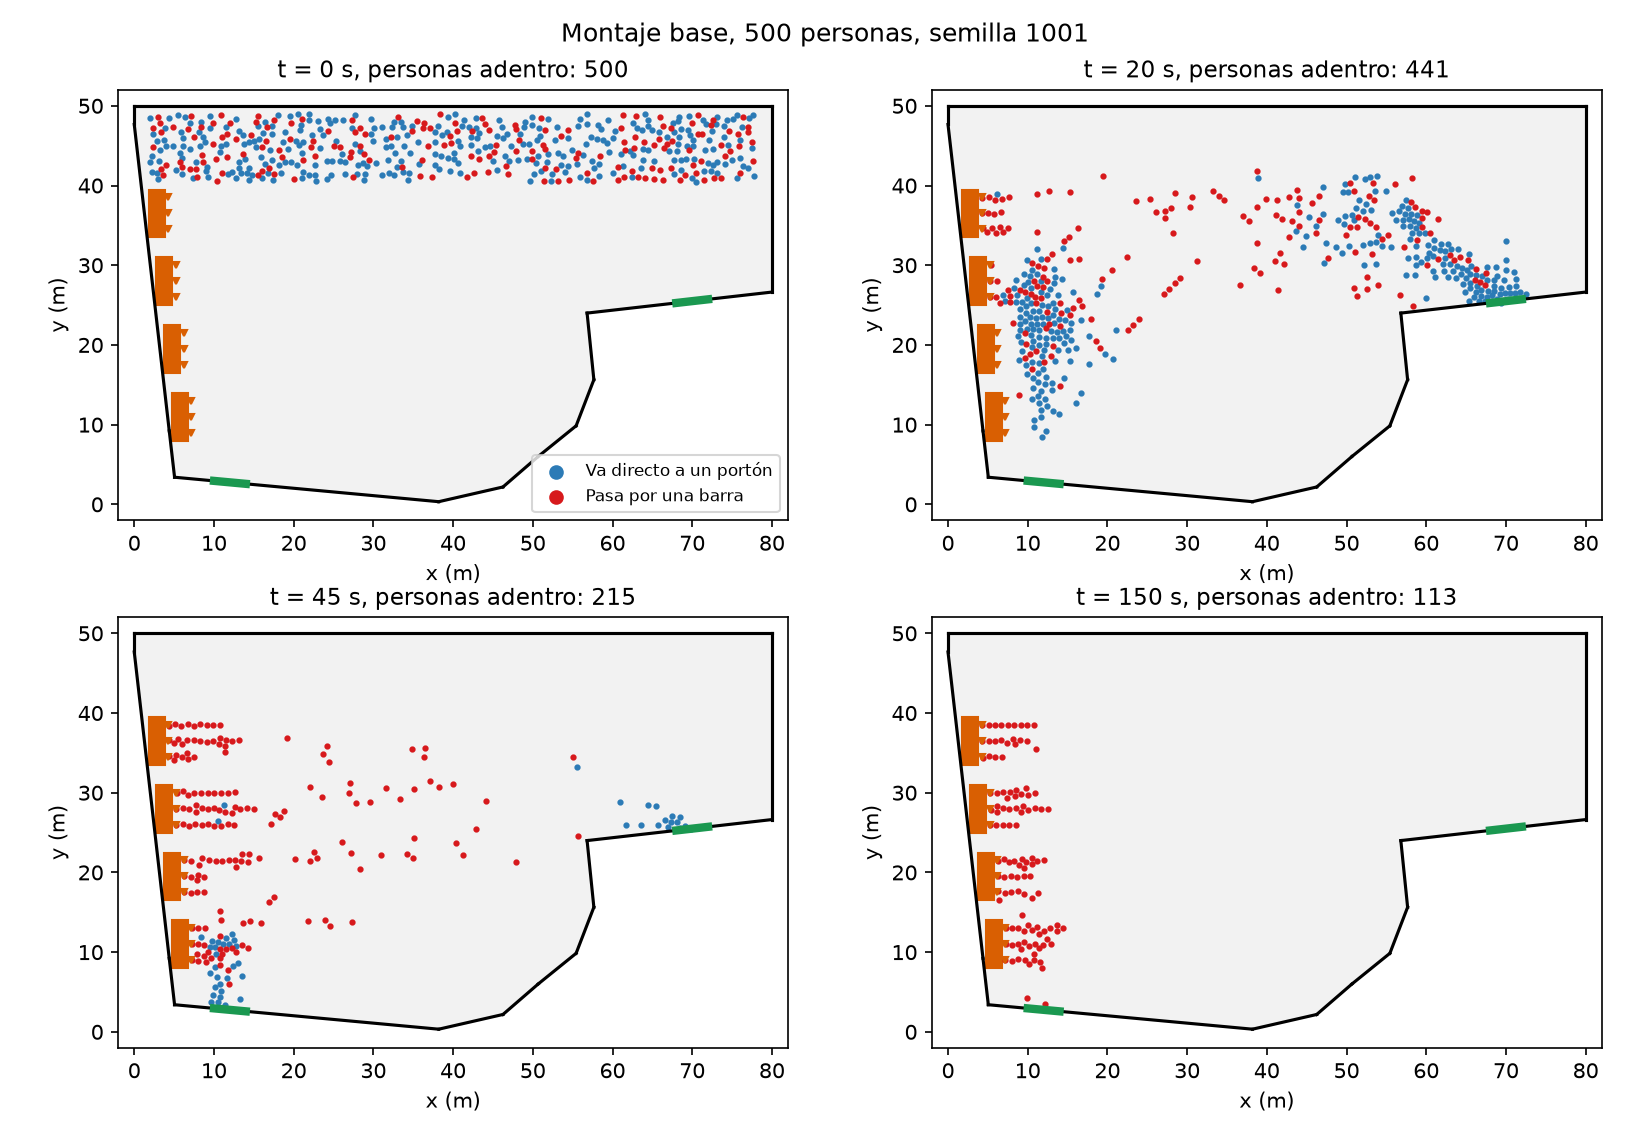
\includegraphics[width=\textwidth]{fig_instantaneas.png}
\caption{Cuatro momentos de una corrida del montaje base con 500 personas.}
\label{fig:instantaneas}
\end{figure}

\subsection{Verificación}
Se automatizaron tres pruebas (\texttt{tests/test\_verification.py}):
\begin{enumerate}
\item \textbf{Conservación}: en cada registro se cumple $N_{\text{adentro}} + N_{\text{evacuados}} = N$ y al final salen todos.
\item \textbf{Muros}: con el montaje base y con uno que incluye vallas, ningún paso de ninguna persona cruza un muro, ninguna posición queda fuera del recinto y la distancia mínima a un muro nunca es menor que el radio de las personas.
\item \textbf{Flujo libre}: una persona sola, que parte del reposo en un pasillo amplio, debe tardar lo que da la solución exacta sin repulsiones, $x(t) = v^0 t - v^0 \tau (1 - e^{-t/\tau})$.
\end{enumerate}

\begin{table}[H]
\centering
\caption{Resultados de las pruebas de verificación.}
\label{tab:verificacion}
\begin{tabular}{lr}
\toprule
Prueba & Resultado \\
\midrule
Conservación: mayor error en N adentro + N evacuados - N & 0 \\
Conservación: todos salen & sí \\
Muros (base): cruces de muro & 0 \\
Muros (base): distancia mínima a un muro (m) & 0.334 \\
Muros (base): posiciones fuera del recinto & 0 \\
Muros (con vallas): cruces de muro & 0 \\
Muros (con vallas): distancia mínima a un muro (m) & 0.312 \\
Muros (con vallas): posiciones fuera del recinto & 0 \\
Flujo libre: tiempo exacto (s) & 41.769 \\
Flujo libre: tiempo simulado (s) & 41.8 \\
Flujo libre: diferencia (s) & 0.031 \\
\bottomrule
\end{tabular}

\end{table}

\printbibliography[title={Referencias}]

\end{document}
